\documentclass[a4paper,14pt]{extarticle}
\usepackage[utf8]{inputenc}
\usepackage[T1,T2A]{fontenc}
\usepackage[english,russian]{babel}

\usepackage{amsthm}
\usepackage{graphicx}
\usepackage{caption}
\usepackage{amssymb}
\usepackage{amsmath}
\usepackage{mathrsfs}
\usepackage{euscript}
\usepackage{graphicx}
\usepackage{subfig}
\usepackage{caption}
\usepackage{color}
\usepackage{bm}
\usepackage{tabularx}
\usepackage{adjustbox}


\usepackage[toc,page]{appendix}

\usepackage{comment}
\usepackage{rotating}

\DeclareMathOperator*{\argmax}{arg\,max}
\DeclareMathOperator*{\argmin}{arg\,min}
\DeclareMathOperator{\E}{\mathbb{E}}

\newtheorem{theorem}{Теорема}
\newtheorem{lemma}[theorem]{Лемма}
\newtheorem{definition}{Определение}[section]

\numberwithin{equation}{section}

\newcommand*{\No}{No.}

\begin{document}

% Титульный лист
%\input{./frontpage.tex}

% Аннотация
\newpage


\begin{abstract}
В данной работе исследуется способ уменьшения размерности пространства обучаемых параметров в задаче детектирования ai текстов, задача многоклассовой классификации. Для fine tuning использовалась модель RoBerta с LoRA адаптером. Было проведено несколько экспериментов, чтобы выяснить, является ли использование LoRA для аппроксимации матрицы весов эффективным с точки зрения времени, ресурсов или точности. Было показано, что при меньших ресурсах модель distilled RoBerta base с LoRA адаптером может получить те же показатели метрик  для классификации текстов, написанных человеком, что и vanilla distilled RoBerta base на наборе данных с 4 классами.


\smallskip
\textbf{Ключевые слова}:  машинное обучение; линейная алгебра; аппроксимация матриц; уменьшение размерности пространств; классификация AI текстов; многоклассовая классификация текстов; большие языковые модели.
\end{abstract}

% Нумерация должна начинаться со второй страницы
\setcounter{page}{2}

% Оглавление
\newpage
\tableofcontents

% Обозначения и сокращения
% \input{./dict.tex}

% Введение
\newpage


\section{Введение}
\paragraph{Актуальность} 
    Уменьшение размерности пространства обучаемых параметров в задаче адаптации к домену упрощает процесс обучения и улучшает вычислительную эффективность. Путем сокращения количества параметров, которые необходимо обновить во время обучения, модель может потенциально быстрее сходиться и затрачивать меньше вычислительных ресурсов; это связано с структурой нейронной сети - ее сложность и потребление ресурсов зависят от количества обучаемых параметров. Уменьшение размерности может быть особенно важным в сценариях адаптации области, где обрабатываются большие объемы данных и происходит обучение с большим числом параметров.
    
\paragraph{Анализ методов решения задачи понижения размерности пространства обучаемых параметров}
    Методы, направленные на решение проблемы снижения размерности: метод главных компонент~\cite{wold1987principal} и его адаптации: тензорное разложение~\cite{oseledets2011tensor},~\cite{qazi2024gpt}, каноническое полиадическое разложение~\cite{zare2018extension} выбирают наиболее важные векторы признаков из набора данных, используя сингулярное разложение матрицы для нахождения первых K собственных векторов с наибольшим собственным значением. Методы, осуществляющие отбор признаков: регуляризация LASSO (L1)~\cite{fonti2017feature}, оценка Фишера~\cite{gu2012generalized} или Тест Хи-квадрат~\cite{zhai2018chi}. Метод снижения размерности, основанный на дообучении больших текстовых моделей - дистилляция~\cite{hsieh2023distilling}; в этом методе большая генеративная модель является «учителем», а меньшая - «учеником». Модель «ученика» обучают с использованием прогнозов "учителя". Эти идеи были впервые представлены в работах Дж. Хинтона~\cite{hinton2015nips} и В.Н. Вапника~\cite{vapnik2015learning}.

    Метод, рассмотренный в данной работе - низкоранговое разложение(англ. Low Rank Adaptation)~\cite{hu2021lora}, который разработан на основе идеи о том, что предварительно обученные языковые модели имеют низкую "внутреннюю размерность" и могут эффективно обучаться, несмотря на проецирование на меньшее подпространство~\cite{aghajanyan2020intrinsic}. Данный метод, как и метод главных компонент, использует сингулярное разложение матрицы для нахождения низкоранговых приближений матрицы весов. 

    Здесь, метод LoRA применяется к одной из наиболее ресурсозатратных задач: обнаружение текстов, написанных искуственным интеллектом(или человеком).
    Проблема обнаружения текстов, написанных искусственным интеллектом, не теряет популярности с годами в научном сообществе. Особенно сейчас, когда отличить тексты, написанные человеком, от текстов, написанных искусственным интеллектом, является основной проблемой для агентств по борьбе с плагиатом. В данной статье мы работали над fine tuning'ом популярной LLM RoBerta с использованием LoRA адаптеров с целью понижения размерности пространства обучаемых параметров. Предполагается, что LoRA может быть так же эффективен в решении задач классификации, как и в задачах генерации: LoRA доказала свою эффективность во многих задачах генерации~\cite{dettmers2024qlora},~\cite{hu2021lora},~\cite{dai2024instructblip}.

\paragraph{Анализ методов решения задачи классификации ai текстов}
Как отмечено в работах~\cite{he2023mgtbench} и~\cite{abdali2024decoding}, все подходы к решению задачи классификации ai текстов, разделяются на два типа: ориентированные на анализ признакового пространства и ориентированные на дообучение моделей. 

1) \textbf{Анализ признакового пространства} основывается на извлечении и анализе характеристик текста - лексических, синтаксических, семантических или стилистических характеристик:~\cite{liang2023gpt},~\cite{yu2023gpt},~\cite{yang2023dna}.


2) \textbf{Дообучение больших языковых моделей} основывается на изучении параметров и возможностей модели и последующем дообучении модели на данных к задаче классификации текстов:~\cite{wolf2019huggingface},~\cite{wolf2019huggingface},~\cite{qasim2022fine}.


\paragraph{Цели}
Исследование снижения пространства обучаемых параметров при помощи разложения матриц.

\paragraph{Методы}
Низкоранговое разложение(англ. Low Rank Adaptation) матриц параметров в больших языковых моделях.

\paragraph{Теоретическая значимость}
В работе проведен теоретический анализ проблемы снижения размерности пространства обучаемых параметров. Доказана теорема об применимости модели BERT~\cite{vaswani2017attention} с адаптером LoRA к задаче многоклассовой классификации. 

\paragraph{Практическая значимость}
Проведен вычислительный эксперимент, показывающий улучшение качества и экономию ресурсов при решении задачи классификации текстов.


% Постановка задачи классификации текстов
\newpage


\section{Постановка задачи классификации текстов}
Модель трансформера решает задачу генерации последовательность в последовательность~(англ. seq2seq), которая формулируется следующим образом согласно~\cite{thickstun2021transformer}: 
\begin{align}
f_\theta: \mathbb{R}^{n \times d} \rightarrow \mathbb{R}^{n \times d},   
\end{align}
где модель~$f_{\theta}$ отображает неупорядоченный набор из~$n$ элементов в~$\mathbb{R}^{d}$ в другой неупорядоченный набор из $n$ элементов в~$\mathbb{R}^{d}$. Для решения задачи классификации текстов(?) сформулируем постановку задачи.
\begin{align}
f_\theta : \hat{V} \rightarrow [N_c],
\end{align}
где~$\hat{V} \subset V^{*}$; $V$~--- словарь токенов и~$V^{*}$~--- его замыкание или множество всех последовательностей над~$V$,~$[N_c]$~--- множество классов. Таким образом, модель отображает текст из~$\hat{V}$ в класс из~$[N_c]$.

Тогда~$(X_i, c_i) \in \hat{V} \times [N_c]$ для~$i \in [N_{data}]$ является парой текст~---класс, выбранной из~$P(X, c)$, где~$X_i$~--- входной текст, а~$c_i$~--- его класс. Таким образом, наша цель~--- оценить~$P(c|X)$.

Согласно~\cite{hu2021lora} при дообучении модель инициализируется предварительно обученными весами~$\Phi_0$ и обновляется до~$\Phi_0 + \Delta\Phi$, где $\Delta\Phi$~--- набор дообучаемых параметров такой, что~$\mid\Delta\Phi\mid = \mid\Phi_0\mid$. Тогда задача минимизации функции потерь имеет вид:
\begin{equation}
\label{eq:12} 
\begin{aligned}
\min _{\Phi}~(-\sum_{X_i \in \hat{V} \subset V^{*}} \sum_{c_i \in [N_c]} \log \left(P_{\Phi}\left(c_i \mid X_i\right)\right)) =\\ 
= \max _{\Phi} \sum_{X_i \in \hat{V} \subset V^{*}} \sum_{c_i \in [N_c]} \log \left(P_{\Phi}\left(c_i \mid X_i\right)\right),
\end{aligned}
\end{equation}
В то время как при использовании LoRA~$\Delta\Phi$ задается набором параметров~$\Theta$ намного меньшего размера:~$\Delta\Phi = \Theta$, где~$\mid\Theta\mid \ll \mid\Phi_0\mid$ и задача минимизации функции потерь имеет вид:
\begin{equation}
\label{eq:13}
\begin{aligned}
\min _{\Theta}~(-\sum_{X_i \in \hat{V} \subset V^{*}} \sum_{c_i \in [N_c]} \log \left(P_{\Phi_0+\Theta}\left(c_i \mid X_i\right)\right)) =\\
= \max _{\Theta} \sum_{X_i \in \hat{V} \subset V^{*}} \sum_{c_i \in [N_c]} \log \left(P_{\Phi_0+\Theta}\left(c_i \mid X_i\right)\right). 
\end{aligned}
\end{equation}




% Предложенный метод
\newpage

\section{Предложенный метод и его корректность}
В данной работе LoRA применяется к задаче классификации. Структура обновления весов при использовании LoRA адаптера описана в таблице~\ref{table:1},
\begin{table}[ht!]
    \centering
\begin{tabular}{ | c | c| } 
 \hline
  Fine tuning & LoRA fine tuning\\ 
 \hline
 $W_{upd} = W + \Delta W$ & $W_{upd} = W + AB$\\ 
 $\hat{y} = xW_{upd}= x(W + \Delta W)$ & $\hat{y} = xW_{upd}= x(W + AB)$\\
 $\hat{y} = xW + x\Delta W$ & $\hat{y} = xW + xAB$ \\
 \hline
\end{tabular}
    \caption{Структура обновления весов при использовании LoRA адаптера}
    \label{table:1}
\end{table}

где~$W \in \mathbb{R}^{d \times k}$~--- предобученные веса,~$\Delta W \in \mathbb{R}^{d \times k}$~--- матрица обновленных весов.~$\Delta W$ приближается с помощью метода LoRA произведением~$AB$, где~$A \in \mathbb{R}^{d \times r}$,~$B \in \mathbb{R}^{r \times k}$ и~$r$~--- ранг матрицы, являющийся гиперпараметром модели. Здесь~$A \sim \mathcal{N}(0,\,\sigma^{2})$ и~$B = [0]_{r \times k}$. 

\subsection{Состоятельность предложенной модели}
Состоятельность модели трансформер была доказана в работе~\cite{lee2023mathematical}. Доказательство приведено для задачи классификации:
\begin{theorem}
\label{theorem:1}
Будем считать, что: 
\begin{enumerate}
    \item Задана модель с набором параметров~$\Theta^*$, генерирующая эмпирическое распределение данных~$P_{model}(\cdot, \Theta^*)$, которое аппроксимирует истинное распределение данных~$P_{true}$ с минимальным расхождением по KL-дивергенции: 
    \begin{equation}
    \label{eq:1}
    \exists \Theta^*: \Theta^* = \argmin _\Theta D_{KL}(P_{true} \mid\mid P_{model}(\cdot, \Theta)),
    \end{equation}
     \item При увеличении размера выборки~$\hat{V}$ эмпирическое распределение данных $P_{model}(\cdot, \Theta^*)$ приближается к истинному распределению, генерирующему данные.
     \item Функция ошибки~$\mathscr{L}(\Theta)$~--- непрерывная, дифференцируемая. Где
\end{enumerate}
\begin{equation}
\label{eq:2.1}
\mathscr{L}(\Theta) = -\frac{1}{\mid \hat{V} \mid}\sum_{X_i \in \hat{V}} \sum_{c_i \in [N_c]} \log \left(P_{\Phi_0+\Theta}\left(c_i \mid X_i\right)\right).
\end{equation}

Тогда минимизация функции потерь~$\mathscr{L}(\Theta)$ приводит к состоятельной оценке истинного распределения, порождающего данные. Т.е.: 
\begin{equation}
\label{eq:2.2}
    \lim_{\mid\hat{V}\mid\to\infty} \argmin _\Theta \mathscr{L}(\Theta) = \Theta^*.
\end{equation}

\end{theorem}
\renewcommand\qedsymbol{$\blacksquare$}
\begin{proof}
В силу равномерной сходимости функции потерь и силу утверждения~\ref{statement:1} из статьи~\cite{donini2018empirical}, которое приведено в приложении:
минимум~$\mathscr{L}(\Theta)$ стремится к минимуму ожидаемого риска~\begin{equation}
    R_{exp}=\E _{X_i \sim P_{true}} [\mathscr{L}(X_i; \Theta)],
\end{equation}при размере $\hat{V}$ стремящемся к бесконечности:
\begin{equation}
\label{eq:3.1}
\begin{aligned}
\lim_{\mid\hat{V}\mid\to\infty}  \argmin _\Theta \mathscr{L}(\Theta)  = \argmin _\Theta R_{exp} = \argmin _\Theta \E _{X_i \sim P_{true}} [\mathscr{L}(X_i; \Theta)].
\end{aligned}
\end{equation}
Достаточно доказать 
\begin{equation}
\label{eq:3.2}
\begin{aligned}
\argmin _\Theta \E _{X_i \sim P_{true}} [\mathscr{L}(X_i; \Theta)] = \Theta^*.
\end{aligned}
\end{equation}
Подставим значение функции потерь:
\begin{equation}
\label{eq:3.3}
\begin{aligned}
\argmin _\Theta \E _{X_i \sim P_{true}} [\mathscr{L}(X_i; \Theta)] =&\\
\argmin _\Theta \E _{X_i \sim P_{true}}[\sum_{c_i \in [N_c]} \log \left(P_{\Phi_0+\Theta}\left(c_i \mid X_i; \Theta)\right]\right).
\end{aligned}
\end{equation}

В силу определения KL-дивергенции,
\begin{equation}
\label{eq:4}
D_{KL}(P || Q)=\int_{-\infty}^{\infty} p(x) \log \left(\frac{p(x)}{q(x)}\right) dx = \E _{x \sim p(x)}[\log \left(\frac{p(x)}{q(x)}\right)],
\end{equation}
верно
\begin{equation}
\label{eq:3.4}
\begin{aligned}
\argmin _\Theta \E _{X_i\in P_{true}}[\sum_{c_i \in [N_c]} \log \left(P_{\Phi_0+\Delta \Phi(\Theta)}\left(c_i \mid X_i\right)\right] =&\\
    \argmin _\Theta D_{KL}(P_{true}\mid\mid P_{model}(\Theta)) =&~\Theta^*,
\end{aligned}
\end{equation}
Последнее равенство справедливо по условию. И оценка \begin{equation}
  \argmin _\Theta \E \mathscr{L}(\Theta)~\textrm{является состоятельной оценкой распределения}~P_{true}.  
\end{equation}
\end{proof}

\subsection{О применимости LoRA к задаче классификации}
Докажем, что LoRA применима к задаче классификации. Для решения задачи классификации с помощью BERT~\cite{vaswani2017attention} требуется не более чем дополнительный~$\operatorname{softmax}$ слой после BERT~\cite{sun2019fine}: 
\begin{equation}
\label{eq:5}
\begin{aligned}
p(c \mid \mathbf{x})&=\operatorname{softmax}(W^T \mathbf{x})\\
\hat{\mathbf{y}}&=\operatorname{softmax}\left(W^T \mathbf{x}\right)=\frac{\exp \left(W^T \mathbf{x}\right)}{\sum_{i=1}^k \exp \left(W^T \mathbf{x}\right)_i},
\end{aligned}
\end{equation}
где~$\mathbf{x}$~--- это выходной результат последнего слоя BERT, а $W$~--- матрица весов.
\begin{figure}[ht!]
    \centering
    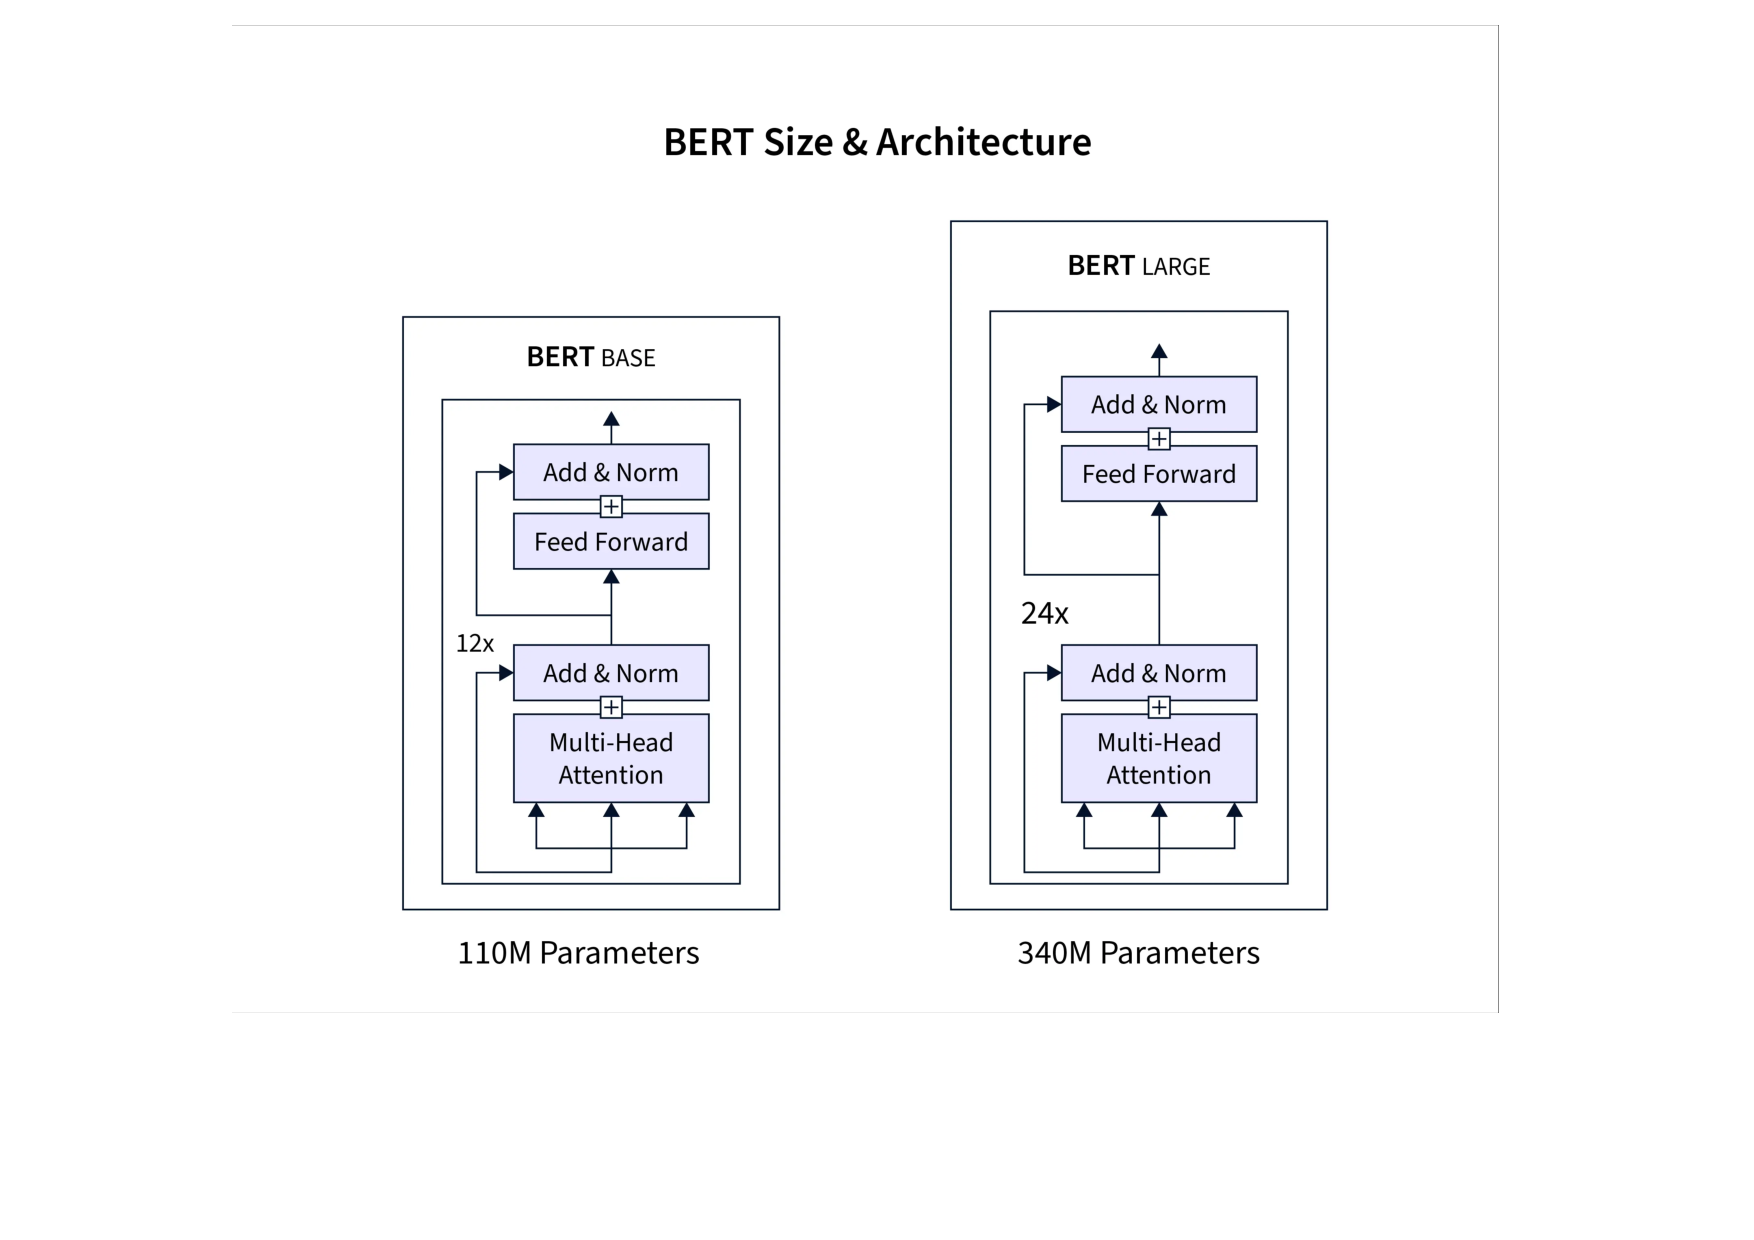
\includegraphics[width=1.0\textwidth]{images/bert_architecture copy.pdf}
    \caption{Архитектура модели BERT}
    \label{fig:1}
\end{figure}
Структура BERT представлена на рис.~\ref{fig:1}, где, согласно~\cite{thickstun2021transformer}, слой внимания~(англ. attention):
\begin{equation}
\begin{aligned}
Q^{(h)}\left(\mathbf{x}_i\right)&=W_{h, q}^T \mathbf{x}_i,\\
K^{(h)}\left(\mathbf{x}_i\right)&=W_{h, k}^T \mathbf{x}_i,  \quad W_{h, q}, W_{h, k}, W_{h, v} \in \mathbb{R}^{d \times k},\\
V^{(h)}\left(\mathbf{x}_i\right)&=W_{h, v}^T \mathbf{x}_i,
\end{aligned}
\end{equation}
\begin{equation}
\begin{aligned}
\alpha_{i,j}^{(h)}=&\operatorname{softmax}_j\left(\frac{\left\langle Q^{(h)}\left(\mathbf{x}_i\right), K^{(h)}\left(\mathbf{x}_j\right)\right\rangle}{\sqrt{k}}\right)V^{(h)}\left(\mathbf{x}_j\right), \\
\mathbf{u}_i^{\prime}=&\sum_{h=1}^H W_{c, h}^T \sum_{j=1}^n \alpha_{i, j}^{(h)}, \\
\end{aligned}
\end{equation}
где $Q^{(h)}\left(\mathbf{x}_i\right), K^{(h)}\left(\mathbf{x}_i\right), V^{(h)}\left(\mathbf{x}_i\right)$~--- линейные проекции входного вектора $\mathbf{x}$ запрос, ключ, значение~(англ. Query, Key, Value) и $\alpha_{i,j}^{(h)}$~--- вектор внимания, $\mathbf{u}_i^{\prime}$~--- выходная матрица слоя attention такого же размера, как и входная $\mathbf{x}_i$~\cite{vaswani2017attention}.

Нормализация по слою~(англ. Layer normalization)~--- нормализует активации предыдущего слоя для каждого входа в партиции~(англ. batch) независимо друг от друга, а не по всей партиции, как при batch нормализации. То есть, применяет преобразование, которое поддерживает среднее в пределах каждого входа близким к 0 и стандартное отклонение активации близким к 1~\cite{ba2016layer}.
\begin{equation}
\begin{aligned}
&\mathbf{u}_i=\operatorname{LayerNorm}\left(\mathbf{x}_i+\mathbf{u}_i^{\prime} ; \gamma_1, \beta_1\right), \\
\end{aligned}
\end{equation}
Нормализация по слою может быть переписана в соответствии с~\cite{ba2016layer} следующим образом:
\begin{equation}
\begin{aligned}
& \operatorname{LayerNorm}(\mathbf{z} ; \gamma, \beta)=\gamma \frac{\left(\mathbf{z}-\mu_{\mathbf{z}}\right)}{\sigma_{\mathbf{z}}}+\beta, \\
& \gamma, \beta \in \mathbb{R}^k . \\
& \mu_{\mathbf{z}}=\frac{1}{k} \sum_{i=1}^k \mathbf{z}_i, \quad \sigma_{\mathbf{z}}=\sqrt{\frac{1}{k} \sum_{i=1}^k\left(\mathbf{z}_i-\mu_{\mathbf{z}}\right)^2} . \\
&
\end{aligned}
\end{equation}
Сеть прямого распространения~(англ. Feed Forward Network) представляет собой двухслойную нейронную сеть с активацией ReLU:
\begin{equation}
\begin{aligned}
& \mathbf{z}_i^{\prime}=W_2^T \operatorname{ReLU}\left(W_1^T \mathbf{u}_i + b_1\right) + b_2. \\
\end{aligned}
\end{equation}
%пояснить!
Нормализация по слою:
\begin{equation}
\begin{aligned}
\mathbf{z}_i=\text { LayerNorm }\left(\mathbf{u}_i+\mathbf{z}_i^{\prime} ; \gamma_2, \beta_2\right) \text {, }
\end{aligned}
\end{equation}


\begin{theorem}
В рамках задачи классификации, при заданных условиях:
\begin{enumerate}
    \item Модель семейства BERT с указанной выше математической структурой и дополнительным слоем 
    \begin{equation}
    \label{eq:6}
        \hat{\mathbf{y}}=\operatorname{softmax}\left(W_{upd}^T \mathbf{x}\right)=\frac{\exp \left(W_{upd}^T \mathbf{x}\right)}{\sum_{i=1}^k \exp \left(W_{upd}^T \mathbf{x}\right)_i},
    \end{equation}
    где 
    \begin{equation}
    \label{eq:7}
    W_{upd} =\underset{(d \times k) }{W} + \underset{(d \times k)}{\Delta W},
    \end{equation}
    и~$x$~---это выходной результат BERT,~$W$~--- матрица весов,~$\Delta W$~--- матрица обновленных весов.
    \item  Данная модель BERT без дополнительного слоя также корректно работает с аппроксимацией 
    \begin{equation}
    \label{eq:8}
    \underset{(d \times k)}{\Delta W} = \underset{(d \times r)}{ A} \times \underset{(r \times k)}{B},
    \end{equation}
    \item Условия теоремы выполняются~\ref{theorem:1}.~(можно считать данную модель состоятельной).
\end{enumerate}
Тогда можно утверждать, что при~\eqref{eq:8} заданная модель BERT с дополнительным слоем гарантирует корректную выходную матрицу.
\end{theorem}
\renewcommand\qedsymbol{$\blacksquare$}
\begin{proof} 
Докажем, что выход из дополнительного слоя корректен. По дистрибутивному свойству сложения матриц и ассоциативному свойтсву произведения матриц: 
\begin{equation}
\label{eq:9}
\begin{aligned}
\hat{\mathbf{y}} = \operatorname{softmax}\left(W_{upd}^T \mathbf{x}\right) =
\operatorname{softmax}\left((W + \Delta W)^T \mathbf{x}\right) =\\ \\
= \frac{\exp \left(W^T \mathbf{x} + \Delta W^T \mathbf{x}\right)}{\sum_{i=1}^k \exp \left(W^T \mathbf{x} + \Delta W^T \mathbf{x}\right)_i}=\\ \\
= \frac{\exp \left(W^T \mathbf{x}\right) \exp \left(\Delta W^T \mathbf{x}\right)}{\sum_{i=1}^k \exp \left(W^T \mathbf{x}\right)_i \exp \left(\Delta W^T \mathbf{x}\right)_i},
\end{aligned}
\end{equation} 
где~$\mathbf{x}$~--- выходная матрица последнего слоя BERT.~$\mathbf{x}$ корректна по условию. В предложенной модели с использованием LoRA:
\begin{equation}
\label{eq:10}
\begin{aligned}
\hat{\mathbf{y}} = \operatorname{softmax}\left(W_{upd} \mathbf{x}\right) =
\operatorname{softmax}\left((W + AB)^T \mathbf{x}\right) =\\ \\
= \frac{\exp \left(W^T \mathbf{x} + (AB)^T \mathbf{x}\right)}{\sum_{i=1}^k \exp \left(W^T \mathbf{x} + (AB)^T \mathbf{x}\right)_i}=\\ \\
= \frac{\exp \left(W^T \mathbf{x}\right) \exp \left((AB)^T \mathbf{x}\right)}{\sum_{i=1}^k \exp \left(W^T \mathbf{x}\right)_i \exp \left((AB)^T \mathbf{x}\right)_i},
\end{aligned}
\end{equation} 
где~$\mathbf{x}$ также выходная матрица BERT с LoRA и~$\mathbf{x}$ корректна по условию. 

Так как финальные размерности остались неизменными, как и~$W^T\mathbf{x}$, легко заметить: 
\begin{equation}
\label{eq:11}
\begin{aligned}
 \underset{(k \times d)}{\Delta W^T} \times \mathbf{x} = u\\
(\underset{(d \times r)}{A} \times \underset{(r \times k)}{B})^T \times \mathbf{x} = (\underset{(k \times r)}{B^T} \times \underset{(r \times d)}{A^T}) \times \mathbf{x} = u^*.
\end{aligned}
\end{equation}
Так как~\eqref{eq:10}, можно заключить что~${u^*} = {u}$ и является корретной матрицей, а следовательно предложенная модель работает корректно.
\end{proof}


% Рубрика эксперименты
\newpage


\section{Вычислительный эксперимент}

Открытый исходный датасет для мультиклассовой классификации текстов, написанных человеком и различными языковыми моделями~\cite{semeval2024task8}. Изначально было представлено 6 классов включая человека, но так как обучение на большем датасете требовало больше ресурсов, а основная задача сравнителного анализа - оценить качество предложенного метода при классификации человек vs языковая модель, то количество классов было сокращено до 4: ChatGPT, Davinci, Cohere, Humans. Это не повлияло на выводы, сделанные в данной работе.

Всего в датасете~$47 327$ текстов с разметкой по классам. Средняя длина текста по всему датасету~---~$400$ слов, средняя длина текстов в зависимости от класса представлена в таблице~\ref{table:3}. Средняя длина слова~--- 5 символов. Вес каждого класса~--- безразмерная величина, показывающая насколько несбалансированна выборка и к каким классам применять большие веса. Статистика по весам классов приведена в таблице~\ref{table:2}.
\begin{table}[ht!]
    \centering
    \begin{tabularx}{.75\textwidth} { 
  | >{\raggedright\arraybackslash}X 
  | >{\raggedleft\arraybackslash}X | }
 \hline
 \textbf{имя класса}  & \textbf{вес, б/р}\\
 \hline
 chatGPT & 0.986\\
 \hline
 cohere  & 1.043\\
 \hline
 davinci & 0.986\\
 \hline
 human & 0.986\\
 \hline
\end{tabularx}
    \caption{Вес каждого класса}
    \label{table:2}
\end{table}
\begin{table}[ht!]
    \centering
    \begin{tabularx}{.75\textwidth} { 
      | >{\raggedright\arraybackslash}X 
      | >{\raggedleft\arraybackslash}X | }
     \hline
     \textbf{имя класса}  & \textbf{длина текста, слова}\\
     \hline
     chatGPT & 362\\
     \hline
     cohere  & 279\\
     \hline
     davinci & 343\\
     \hline
     human & 607\\
     \hline
    \end{tabularx}
    \caption{Средняя длина текста}
    \label{table:3}
\end{table}

Заметим, что текст, написанный человеком, в среднем в 2-3 раза длиннее написанного машиной. При этом средняя длина слова для каждого класса одна и та же~--- 5 символов. Тексты были токенизированы при помощи RobertaTokenizer~\cite{wolf2019huggingface}, токенизатора использующего пары байтов для кодировки~(англ. Byte-Pair Encoding)~\cite{wang2020neural}. Дополнительная обработка не требуется из-за структуры модели~\cite{vaswani2017attention}. Для всех экспериментов использовалась предобученная модель DistilRoBERTa base~\cite{liu2019roberta}. Модель использовалась со следующими гиперпараметрами: доля тренировочного/тестового набора данных~---~$0.9/0.1$; 3 эпохи обучения. Для экспериментов с использованием алгоритма LoRA были использованы все вышеуказанные параметры, а также ранг матриц аппроксимации~$r = 5$.

После обучения для оценки использовались матрица ошибок и метрики точности, полноты, F1-меры, а также для визуализации ошибки использовалась матрица ошибок~(англ. Confusion matrix) как наиболее точно отображающие качетво моделей мультиклассовой классификации~\cite{grandini2020metrics}. В матрице ошибок по вертикали указаны истинные метки классов, а по горизонтали~--- предсказанные.

\subsection{Предобученная модель DRoBERTa-base, мультиклассовая классификация.}
Результаты обучения данной модели представлены в таблице~\ref{table:4}. Для наглядного описания качества модели используется матрица ошибок: таблица~\ref{table:5}.
\begin{table}[ht!]
    \centering
    \begin{tabularx}{\textwidth} { 
      | >{\raggedright\arraybackslash}X 
      | >{\centering\arraybackslash}X 
      | >{\centering\arraybackslash}X 
      | >{\raggedleft\arraybackslash}X | }
     \hline
     \textbf{имя класса}  & \textbf{precision} & \textbf{recall} & \textbf{f1-score}\\
     \hline
     chatGPT & 1.000 & 0.993 & 0.997\\
     \hline
     cohere  & 0.963  & 0.999 & 0.981\\
     \hline
     davinci & 0.986 & 0.996 & 0.991\\
     \hline
     human & 0.991 & 0.952 & 0.971\\
     \hline
    \end{tabularx}
    \caption{Метрики качетва DRoBERTa-base}
    \label{table:4}
\end{table}
\begin{table}[ht!]
\centering
\begin{tabular}{ cc|c|c|c|c }
    && chatGPT & Cohere & Davinci & Human \\ \cline{2-6}
    & chatGPT & \cellcolor{cobalt}{\textcolor{white}{\textbf{0.993}}} & \cellcolor{bubbles}{0.002} & \cellcolor{bubbles}{0.0} & \cellcolor{bubbles}{0.005} \\ \cline{2-6}
    & Cohere & \cellcolor{bubbles}{0.0} & \cellcolor{cobalt}{\textcolor{white}{\textbf{0.999}}} & \cellcolor{bubbles}{0.0} & \cellcolor{bubbles}{0.001} \\ \cline{2-6}
    & Davinci & \cellcolor{bubbles}{0.0} & \cellcolor{bubbles}{0.001} & \cellcolor{cobalt}{\textcolor{white}{\textbf{0.996}}} & \cellcolor{bubbles}{0.003}\\ \cline{2-6}
& Human & \cellcolor{bubbles}{0.0} & \cellcolor{bubbles}{0.035} & \cellcolor{bubbles}{0.013} & \cellcolor{cobalt}{\textcolor{white}{\textbf{0.952}}}\\ 
\end{tabular} 
\caption{Матрица ошибок, DRoBERTa-base}
\label{table:5}
\end{table}
Модель показала высокое качество на уровне 99\%, но потребовала много вычислительных ресурсов: время обучения заняло: 4041.3188 секунд. Построим модель с использованием LoRA, чтобы ускорить обучение и уменьшить ресурсозатратность.

\subsection{Предобученная модель DRoBERTa-base \& LoRA, мультиклассовая классификация.}
Только 0.828\% параметров обучаются при использовании LoRA: \textit{trainable params: 685828, all: 82807304 || trainable\%: 0.8282}, а затраченное время обучения~--- 3210.977 секунд, по сравнению с 4041.3 из первого эксперимента. Но качество модели заметно упало. Это наиболее заметно в классе human: recall составил всего 31,7\%, что отображено в таблице~\ref{table:6}. Матрица ошибок также демонстрирует разкое ухудшение метрик;матрица ошибок для данноого эксперимента представлена в таблице~\ref{table:7}.
\begin{table}[ht!]
    \centering
    \begin{tabularx}{\textwidth} { 
      | >{\raggedright\arraybackslash}X 
      | >{\centering\arraybackslash}X 
      | >{\centering\arraybackslash}X 
      | >{\raggedleft\arraybackslash}X | }
     \hline
     \textbf{model}  & \textbf{precision} & \textbf{recall} & \textbf{f1-score}\\
     \hline
     chatGPT & 0.997 & 0.786 & 0.879\\
     \hline
     cohere  & 0.667  & 0.940 & 0.780\\
     \hline
     davinci & 0.703 & 0.971 & 0.816\\
     \hline
     human & 0.717 & 0.317 & 0.440\\
     \hline
    \end{tabularx}
    \caption{Метрики качетва DRoBERTa-base \& LoRA}
    \label{table:6}
\end{table}
\begin{table}[ht!]
\centering
\begin{tabular}{ cc|c|c|c|c }
    \multicolumn{5}{c}{предсказаные метки} \\ 
    \multirow{5}{*}{\rotatebox{90}{истинные метки}} & & chatGPT & Cohere & Davinci & Human \\ \cline{2-6}
    & chatGPT & \cellcolor{bleudefrance}{\textcolor{white}{\textbf{0.79}}} & \cellcolor{bubbles}{0.01} & \cellcolor{bubbles}{0.08} & \cellcolor{babyblue}{0.12} \\ \cline{2-6}
    & Cohere & \cellcolor{bubbles}{0.0} & \cellcolor{ceruleanblue}{\textcolor{white}{\textbf{0.94}}} & \cellcolor{bubbles}{0.06} & \cellcolor{bubbles}{0.003} \\ \cline{2-6}
    & Davinci & \cellcolor{bubbles}{0.001} & \cellcolor{bubbles}{0.03} & \cellcolor{cobalt}{\textcolor{white}{\textbf{0.98}}} & \cellcolor{bubbles}{0.0}\\ \cline{2-6}
    & Human & \cellcolor{bubbles}{0.002} & \cellcolor{babyblueeyes}{0.43} & \cellcolor{babyblueeyes}{0.25} & \cellcolor{babyblueeyes}{{\textbf{0.32}}}\\ 
\end{tabular} 
\caption{Confusion matrix,\\ DRoBERTa-base~\&~LoRA}
\label{table:7}
\end{table}

Метрики качества заметно упали. В большей степени для класса human, который представляет наибольший интерес: в первую очередь важнее всего классифицировать human vs ai, и если текст написала языковая модель, то определять какая. В следующем эксперименте проверим гипотезу: предполагаемая скорость обучения сохранится, а метрики качества вырастут.

\subsection{Три независимые модели DRoBERTa-base \& LoRA, бинарная классификация.}
\textbf{ChatGPT vs Human}\\ 
Эксперимент, представленный здесь, аналогичен предыдущему, но три независимые модели решают задачи бинарной классификации, а потом их результат успедняется. В первой части этого эксперимента рассмотрим классы chatGPT и human. Время обучения сократилось в несколько раз, как и предполагалось, и составило 1633.8114 секунд. Метрики качества также выросли и в среднем составили 95\%. Особенно хоршие результаты показаны на классе human~--- до 100\%. Результаты представлены в таблицах~\ref{table:8},~\ref{table:9}.
\begin{table}[ht!]
    \centering
    \begin{tabularx}{\textwidth} { 
      | >{\raggedright\arraybackslash}X 
      | >{\centering\arraybackslash}X 
      | >{\centering\arraybackslash}X 
      | >{\raggedleft\arraybackslash}X | }
     \multicolumn{4}{c}{\textbf{время обучения: 1633.8114 секунд}} \\
     \hline
     \textbf{model}  & \textbf{precision} & \textbf{recall} & \textbf{f1-score}\\
     \hline
     chatGPT & 1.000 & 0.891 & 0.942\\
     \hline
     human & 0.902 & 1.000 & 0.950\\
     \hline
    \end{tabularx} 
    \caption{Метрики качетва DRoBERTa-base \& LoRA,\\ chatGPT vs Human}
    \label{table:8}
\end{table}

\begin{table}[ht!]
\centering
\begin{tabular}{ cc|c|c }
    & & chatGPT & Human \\ 
    \cline{2-4}
    & chatGPT & \cellcolor{bleudefrance}{\textcolor{white}{\textbf{0.892}}} & \cellcolor{babyblue}{0.108} \\ \cline{2-4}
    & Human & \cellcolor{bubbles}{0.0} & \cellcolor{cobalt}{\textcolor{white}{\textbf{1.00}}}\\ 
\end{tabular} 
\caption{Матрица ошибок,\\ DRoBERTa-base~\&~LoRA, chatGPT vs Human}
\label{table:9}
\end{table} 
\textbf{Cohere vs Human}\\ 
Аналогично, заметен резкий рост в качетсве, в особенности для класса human. Также время обучения значительно сократилось и составило 1583.556 секунд. Выводы аналогичны первой части данного эксперимента. Результат представлен в таблице~\ref{table:10} и матрица ошибок представлена в таблице~\ref{table:11}.
\begin{table}[ht!]
    \centering
    \begin{tabularx}{\textwidth} { 
      | >{\raggedright\arraybackslash}X 
      | >{\centering\arraybackslash}X 
      | >{\centering\arraybackslash}X 
      | >{\raggedleft\arraybackslash}X | }
      \multicolumn{4}{c}{\textbf{время обучения: 1583.556 секунд}} \\ 
     \hline
     \textbf{model}  & \textbf{precision} & \textbf{recall} & \textbf{f1-score}\\
     \hline
     cohere & 0.999 & 0.837 & 0.911\\
     \hline
     human & 0.853 & 0.999 & 0.920\\
     \hline
    \end{tabularx}
    \caption{Метрики качетва DRoBERTa-base \& LoRA,\\ Cohere vs Human}
    \label{table:10}
\end{table}
\begin{table}[ht!]
\centering
\begin{tabular}{ cc|c|c }
    & & Cohere & Human \\ 
    \cline{2-4}
    & Cohere & \cellcolor{bleudefrance}{\textcolor{white}{\textbf{0.837}}} & \cellcolor{babyblue}{0.163} \\ \cline{2-4}
    & Human & \cellcolor{bubbles}{0.001} & \cellcolor{cobalt}{\textcolor{white}{\textbf{0.999}}}\\ 
\end{tabular} 
\caption{Матрица ошибок,\\ DRoBERTa-base~\&~LoRA, Cohere vs Human}
\label{table:11}
\end{table} 

\textbf{Davinci vs Human}\\ 
Наблюдения аналогичны предыдущим в рамках эксперимента. Время обучения составило 1632.395 секунд. Результат эксперимента представлен в таблице~\ref{table:12} и матрица несоответсвий представлена в таблице~\ref{table:13}. Если усреднить показатели трех моделей эксперимента, то можно заметить улучшение качества по сравнению с метриками качетва DistilRoBERTa base \& LoRA для мультиклассовой классификации; для класса human recall составил 99\%, для других классов особенно выросла метрика precision~--- до 99\% в среднем, в сравнении с 97\% из первого эксперимента, где к модели DistilRoBERTa base не применялся LoRA адаптер. Результат представлен в таблицах~\ref{table:14} и ~\ref{table:15}.

\begin{table}[ht!]
    \centering
    \begin{tabularx}{\textwidth} { 
      | >{\raggedright\arraybackslash}X 
      | >{\centering\arraybackslash}X 
      | >{\centering\arraybackslash}X 
      | >{\raggedleft\arraybackslash}X | }
    \multicolumn{4}{c}{\textbf{время обучения: 1632.395 секунд}} \\ 
     \hline
     \textbf{model}  & \textbf{precision} & \textbf{recall} & \textbf{f1-score}\\
     \hline
     davinci & 0.996 & 0.851 & 0.918\\
     \hline
     human & 0.870 & 0.997 & 0.929\\
     \hline
    \end{tabularx}
    \caption{Метрики качетва DRoBERTa-base \& LoRA,\\Davinci vs Human}
    \label{table:12}
\end{table}
\begin{table}[ht!]
\centering
\begin{tabular}{ cc|c|c }
    & & Davinci & Human \\ 
    \cline{2-4}
    & Davinci & \cellcolor{bleudefrance}{\textcolor{white}{\textbf{0.852}}} & \cellcolor{babyblue}{0.148} \\ \cline{2-4}
    & Human & \cellcolor{bubbles}{0.003} & \cellcolor{cobalt}{\textcolor{white}{\textbf{0.997}}}\\ 
\end{tabular} 
\caption{Матрица ошибок,\\ DRoBERTa-base~\&~LoRA, Davinci vs Human}
\label{table:13}
\end{table} 

\begin{table}[ht!]
    \centering
    \begin{tabularx}{\textwidth} { 
      | >{\raggedright\arraybackslash}X 
      | >{\centering\arraybackslash}X 
      | >{\centering\arraybackslash}X 
      | >{\raggedleft\arraybackslash}X | }
     \hline
     \textbf{model}  & \textbf{precision} & \textbf{recall} & \textbf{f1-score}\\
     \hline
     chatGPT & 1.000 & 0.891 & 0.942\\
     \hline
     cohere  & 0.999  & 0.837 & 0.911\\
     \hline
     davinci & 0.996 & 0.851 & 0.918\\
     \hline
     human & 0.875 & 0.999 & 0.933\\
     \hline
    \end{tabularx}
    \caption{Метрики качетва DRoBERTa-base \& LoRA, бинарные классификаторы}
    \label{table:14}
\end{table}

\begin{table}[ht!]
    \centering
    \begin{tabularx}{\textwidth} { 
      | >{\raggedright\arraybackslash}X 
      | >{\centering\arraybackslash}X 
      | >{\centering\arraybackslash}X 
      | >{\raggedleft\arraybackslash}X | }
     \hline
      \textbf{model}  & \textbf{precision} & \textbf{recall} & \textbf{f1-score}\\
     \hline
     chatGPT & 1.000 & 0.993 & 0.997\\
     \hline
     cohere  & 0.963  & 0.999 & 0.981\\
     \hline
     davinci & 0.986 & 0.996 & 0.991\\
     \hline
     human & 0.991 & 0.952 & 0.971\\
     \hline
    \end{tabularx}
    \caption{Метрики качетва DRoBERTa-base, мультиклассовая классификация}
    \label{table:15}
\end{table}
Итого, в эксперименте, использующем DistilRoBERTa base \& LoRA для бинарной классификации и последующего усреднения, качество классификации выросло, не потеряв во времени обучения, по сравнению с предобученной моделью DistilRoBERTa base. А также по результатам эксперимента с использованием DistilRoBERTa base \& LoRA для бинарной классификации, модель сильно выиграла в качестве у модели DRoBERTa-base \& LoRA для мультиклассовой классификации, но проиграв ей во времени обучения. 











% Выводы
\newpage

\section{Заключение}
В работе рассматривался метод LoRA снижения размерности пространства обучаемых параметров в задаче классификации текстов, написанных большими языковыми моделями. Была сформулированна и доказана теорема о конструктивности предложенного метода.

В ходе эксперимента на датасете из текстов, написанных как языковыми моделями, так и человеком, была доказана эффективность предложенного метода.
При решении задачи мультиклассовой классификации предложенная модель BERT \& LoRA  тратит меньше ресурсов, чем модель без использования LoRA, но метрики качества падают. Однако, при решении тремя одинаковыми независимыми моделями задачи бинарной классификации с последующим усреднением метрики качетва растут, а использование ресурсов~--- нет. Таким образом, в данной работе теоритически и экспериментально доказана состоятельность и эффективность предложенного метода.



% Библиографические ссылки
\newpage
\bibliographystyle{plain}
\bibliography{ref} 

% Приложения
%\newpage


\begin{lemma}
\label{statement:1}
Утверждение из статьи~\cite{donini2018empirical}:
В терминах постаноки задачи классификации текстов:
для функции риска $L(\Theta)$:
\begin{equation}
\label{eq:2.3}
L(\Theta) = \E _{X_i} \mathscr{L}(X_i; \Theta)
\end{equation}
и функции эмпирического риска $\hat{L}(\Theta)$:
\begin{equation}
\hat{L}(\Theta) = \frac{1}{\mid \hat{V} \mid} \sum_{X_i \in \hat{V}} \mathscr{L}(X_i; \Theta) 
\end{equation}
\text{верно следующее:}
\begin{equation}
\sup _{\Theta} \mid L(\Theta) - \hat{L}(\Theta) \mid \le \delta(\mid \hat{V} \mid):
\end{equation}
\begin{equation}
\delta(\mid \hat{V} \mid) \xrightarrow[\mid \hat{V} \mid \rightarrow \inf]{} 0
\end{equation}
\end{lemma}


\end{document}